\subsection{Extending collaboration tools with time manipulation}

Real time collaboration applications have become a huge help on team tasks, providing a great boost on business, research and investigation velocity. Technologies like these are appearing along these days, but they couldn't be possible years ago because technology was limited or unavailable. Although today's technology is limited on some aspects, we are doing progress in order to improve the web ecosystem, by creating standards and migrating to newer technologies.

 Our first concern on real time collaboration applications, besides the communication itself, is the data storage and representation. Storing multimedia content is not a viable solution because most browsers are recommended to limit local storage to at least five megabytes per origin.

	If, for instance, one wants to rewind a real-time video, recordings will be needed from whom is streaming the video. 

  \ac{RTP}\cite{rfc3550} is used for streaming audio and video over \ac{IP}, the multimedia content is transported on the payload of \ac{RTP} messages, \ac{RTP} contains headers for payload identification. \ac{RTP} is independent from its payload type, allowing to transport any kind of encoded multimedia. A sequence number is used for sorting received packets.

\ac{RTCP} is used for controlling \ac{RTP} multimedia streams, it provides bandwidth statistics and control information that can be used for changing the quality of the stream in real-time.

  \ac{RTP} allows to change its requirements and add extensions to it with profiles, one of the most used is the \ac{RTP} profile for audio and video \cite{rfc3551} which lists the payload encoding and compression algorithms. This profile also assigns a name to each encoding which may be used other protocols like \ac{SDP}.

  Another profile for \ac{RTP} is defined by \ac{SRTP}, which provides encryption, authentication and replay protection of \ac {RTP} traffic. The analogous secure protocol for \ac{RTCP} is \ac{SRTCP}.

  Both \ac{SRTP} and \ac{SRTCP} use \ac{AES} by default, which is symmetric-key algorithm for data encryption. Each packet is encrypted using a distinct key-stream, otherwise using a single key-stream with \ac{AES} on \ac{CBC} would make impossible to recover from packet loss.

  Two key-stream generators for \ac{AES} were defined: \textit{Segmented Integer Counter Mode} and \textit{f8-mode}. If a packet is lost, there is no impact on other packets, as the initialization vector is obtained through those key-stream generators and it's fixed for each packet.

  \ac{RTP} recorders are independent of payload encoding, they don't decode \ac{RTP} packets, they record packets instead, allowing to record all video and audio formats even if they're encrypted.

\begin{figure}[H]
	\centering
	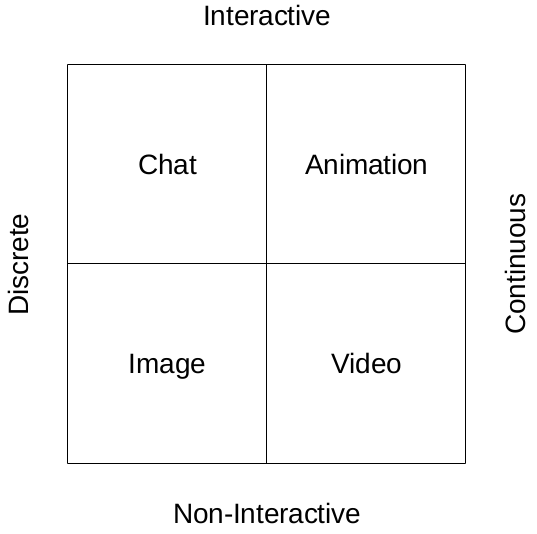
\includegraphics[width=0.45\textwidth]{figures/media_types.png}
	\caption{Media Types}
\end{figure}

	Media Types can be distinguished by two criteria, the first one describes a media as discrete or continuous, the second one describes it as interactive or non-interactive. A discrete media is characterized by its type not depending from time, as continuous media depending from it. Interactive media is characterized by its state being changed by external events such as user interactions.

	For example, an image is non-interactive and discrete, for instance, a video is continuous and non-interactive. A simple collaborative editor with just text is interactive and discrete. An animation that changes in function of user behavior is interactive and continuous.

	Streaming protocols like \ac {RTP} were designed for continuous and non-interactive media types, such as audio and video. Discrete and non-interactive media don't need to be streamed through \ac{RTP} because they don't change with. For example, if an image appears in a specific time interval, just the \ac{HTML} or \textit{JavaScript} that will reference the image must be streamed, the image itself is then transferred through \ac{HTTP}.

	In order to play any kind of stream, a player for interactive stream is needed for downloading an environment, decoding the \ac{RTP} payload to determine the state and display it to the user. Streaming interactive media like the combination of \ac{HTML}, \ac{CSS} and JavaScript require more than interpreting the code, a streamed user interface may contain an internal state that is not shown on code.

	Every time an event is processed on one of the endpoints, both sender and receivers state must stay synchronized, otherwise events may behave differently.

	To achieve synchronization of interactive data most packets have three types: \textit{State}, \textit{Delta-State} and \textit{Event}. State packet defines the environment complete state. Delta-State packets transports just the piece of state that changed. Event packets informs that an event occurred over the interactive media. 


	An \ac{RTP} recorder can have two operation modes, recording or playback. Traditional \ac{RTP} players can do random access, in contrast, interactive \ac{RTP} players must restore the environment and context at a given time. The environment is the initial state, so we can call it a non-interactive discrete media and handle it over \ac{HTTP}. After the receiver has received the environment, it should calculate the state at the given time. 

	If the \ac{RTP} recorder controls the correct data to send to the receivers, it cannot be a simple \ac{RTP} recorder as it must compute the state or delta-state to send. Therefore, if the receiver receives all recorded packets, it can calculate the current state from the previous complete state. Streaming too much complete states, results on more precise random accesses, but the trade-off is the higher bandwidth usage and used storage space on the recording server. On the other hand, if there are fewer complete states recorded followed by delta-states, the recorded stream will occupy less storage space, but random accesses will be less granular.

	It is possible to restore the media state even if messages are lost by recording and streaming the interactive media's complete state periodically.

	In order to synchronize an interactive application state amongst participants, the needed objects to synchronize must be serializable and sent to other participants.

  {\color{fade}[Model View Controller (Suited for interactive RTP)]}

	With such an interactive \ac{RTP} recorder it is then possible to record, play, fast forward, fast rewind, stop and jump to random positions.

  \cite{interactive_stream} proposed an \ac{RTP} profile for real-time transmission of interactive media. This new profile reuses much of video and audio profile implementation, integrating the interactive component.   \cite{interactive_record} explained how to record interactive video with this new profile.
	
	Multi-party video calls can be achieved on \ac{WebRTC} by streaming video from each participant to all the other participants. Although this works, the bigger a conference room is, the bigger is the bandwidth used to stream video to all participants within the conference room.

	\textit{Jitsi Video Bridge} \footnote{\url{http://jitsi.org/Projects/JitsiVideobridge}} receives one stream from every participant on a conference, either from a \textit{jitsi} client or a \ac{WebRTC} application, and redirects it to all the other conference participants, reducing the amount of data that each peer sends. Although all the participants need to download all the streams from \textit{Jitsi Video Bridge} server, typically download rates are much bigger than upload rates, making this solution more feasible.

	\textit{Jitsi Video Bridge} uses \ac{XMPP} as a signaling protocol and its \textit{colibri} extension \cite{xep0340} to reserve channels for video transmission. Although this choice for signaling protocol, \textit{Jitsi Video Bridge} also supports \ac{SIP}.

  {\color{fade}[Identity is that important?]}
